%File: intro.tex
%Date: Thu Jun 26 13:01:10 2014 +0800
%Author: Yuxin Wu <ppwwyyxxc@gmail.com>

\section{项目概述}
\large
\setlength{\baselineskip}{15pt}
\subsection{功能}

如今的研究者在搜索论文中, 在种类繁多的论文资源提供平台中, 常常会遇到跳转过多, 文件名混乱等问题.
\begin{figure}[H]
  \centering
  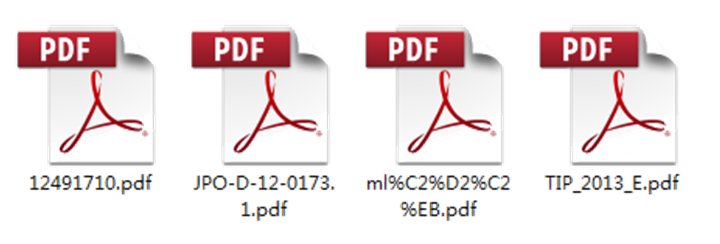
\includegraphics[width=0.7\textwidth]{img/chaos.png}
\end{figure}
\begin{figure}[H]
  \centering
  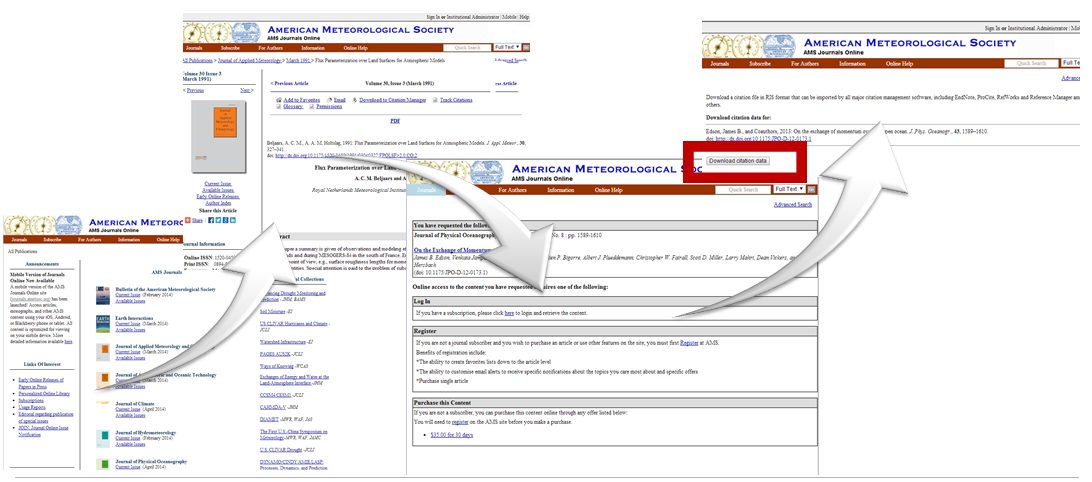
\includegraphics[width=0.7\textwidth]{img/redirect.png}
\end{figure}

搭建一个学术搜索引擎.根据用户输入查询内容(论文的标题、作者、内容摘要等),检索并呈现指定的论文.
在获得版权前提下,提供直接下载链接,并保证下载完成后论文名称正确.

\subsection{文件结构}
\dirtree{%
  .1 /.
  .2 common/\DTcomment{功能及主要逻辑的实现}.
  .3 fetcher/\DTcomment{各论文提供源爬虫}.
  .3 lib/\DTcomment{公共库}.
  .3 searcher/\DTcomment{搜索引擎爬虫}.
  .3 xpengine/\DTcomment{内容数据库引擎}.
  .3 contentsearch.py\DTcomment{内容搜索逻辑实现}.
  .3 dbsearch.py\DTcomment{论文数据库搜索逻辑实现}.
  .3 pdfprocess.py\DTcomment{pdf处理库实现}.
  .3 queryhandler.py\DTcomment{外部请求处理逻辑}.
  .3 test-{fetcher,searcher}.py\DTcomment{fetcher与searcher的测试}.
  .3 job.py\DTcomment{定义查询的任务上下文}.
  .3 ukconfig.py\DTcomment{库功能的配置}.
  .3 ukdbconn.py\DTcomment{与mongo数据库交互的基本功能实现}.
  .3 uklogger.py\DTcomment{日志系统实现}.
  .2 report/\DTcomment{本报告的\LaTeX 源代码}.
  .2 manage/\DTcomment{开发用脚本,用于部署服务,操纵数据库等}.
  .2 webapi/\DTcomment{HTTP服务器实现}.
  .3 api/\DTcomment{RESTful API实现}.
  .3 static/\DTcomment{静态页面资源}.
  .3 templates/\DTcomment{HTML模板}.
  .2 paper-downloader.py\DTcomment{自动搜索下载paper的命令行工具}.
  .2 standalone\_server.py\DTcomment{服务器运行入口}.
}
\subsection{依赖}
运行命令行工具需要如下python包:
\begin{enumerate}
  \item requests \footnote{\url{http://docs.python-requests.org/en/latest/}}
  \item BeautifulSoup4 \footnote{\url{http://www.crummy.com/software/BeautifulSoup/bs4/doc/}}
  \item termcolor \footnote{\url{https://pypi.python.org/pypi/termcolor}}
\end{enumerate}

部署服务器需要系统中除python包外, 拥有如下库或软件:
\begin{enumerate}
  \item Mongodb安装并运行. 可在\verb|common/ukconfig.py|中配置其位置.
  \item python virtualenv
  \item ghostscript
  \item libcurl
  \item xapian
  \item pdf2htmlEx
  \item poppler-utils
\end{enumerate}
\subsection{运行方法}
\begin{enumerate}
    \item 命令行使用爬虫下载paper:
      \begin{lstlisting}[language=bash]
./paper-downloader.py -t "title of the paper" -d /tmp
      \end{lstlisting}

    \item 启动服务器:

通过如下命令安装python包依赖, 并部署虚拟环境:
\begin{lstlisting}[language=bash]
$ cd manage
$ ./quickinstall
\end{lstlisting}

部署后, 通过\verb|./standalone_server.py|直接运行.
服务器配置在\verb|manage/api_website_config.py|中.
\end{enumerate}


\section{后端实现}

\subsection{系统架构}
HTTP服务器使用python的Flask框架实现.
各功能的实现也均使用python.
系统中, HTTP服务器与后台逻辑完全解耦, 因此在不启动服务时仍然可以通过\verb|paper-downloader.py|调用
sopaper爬虫进行论文的搜索,下载, 方便日常使用.

系统后端除服务器外, 主要由三部分构成:Searcher,Parser,Processor.
其中Searcher主要负责将查询送往搜索引擎,
Parser负责对异构的网页及进行解析和抓取资源,
Processor对获取的论文进行展示前的压缩,转码处理.

\subsection{查询处理流程}

当一个查询进入处理后, 会立刻建立一个任务上下文\verb|JobContext|对象.
该对象会依次被各个searcher及parser所更新, 以汇总多方的数据.

例如, 可以利用google / google scholar的结果来对paper的标题进行纠正.
google搜索所提供的citation信息也可以加以利用. 同时, 打开google所提供的搜索结果后,
也可能能够进一步parse出citation信息作为补充.
正是由于不同服务都可能提供不同的数据, 将paper数据全部封装在一个上下文中进行Stream式的处理会使得项目逻辑更加清晰.

在searcher阶段, 查询会被送往搜索引擎, 以寻找互联网上的论文资源. 在parser阶段,
对搜索引擎查找到的异构结果进行解析得到结构化数据.
过程中一旦获得有用的标识, 就会及时查询本地数据库是否已有相应数据, 以免浪费网络流量.
在元信息获取,整合完毕后, 将结果返回给前端, 同时后端开始异步下载并通知前端下载进度.
下载完成后, 对paper进行后处理, 送往前端展示并提供下载链接.

\subsection{插件式爬虫}

所有资源爬虫位于\verb|common/fetcher/|目录下, 爬虫采取插件式设计,
每个爬虫继承自\verb|FetcherBase|,在系统启动时被系统自动发现,
并通过decorator进行自注册.
注册的爬虫实现如下接口:
\begin{enumerate}
  \item 爬虫可处理的url格式
  \item 爬虫可能提供的paper信息
  \item 爬虫优先级
  \item 获取各类paper信息
  \item 下载paper
\end{enumerate}

\subsection{论文后处理}

当获取到paper的pdf原始文件后, 会对其进行如下后处理:
\begin{enumerate}
  \item 压缩:

    使用libpoppler中的工具对pdf进行压缩, 数据库中的所有论文平均压缩至原大小的55\%,
    尤其对于较大的pdf压缩更为明显 (因为较大的pdf大多是由于生成方式不高效导致的).
    压缩使得从sopaper可以下载到更小的论文.

  \item 转HTML:

    使用pdf2htmlEx工具将pdf转为分页HTML, 并存储在数据库中.
    展示时, 由前端发送一个或多个页码的http请求获取html再进行渲染.

  \item 转文本:

    使用libpoppler库将pdf转为纯文本, 用于建立数据索引进行内容搜索.

\end{enumerate}
\subsection{数据库索引及查询}

内容数据库采用xapian的python封装xappy实现.
xapian\footnote{\url{http://xapian.org}}是一个轻量, 高效的搜索引擎后端, 且支持模糊查询, 布尔查询, 多域查询等功能.

xapian默认使用BM25作为结果的相关程度指标, 考虑到paper搜索的特殊性, 还加入了citation等因素综合评判.

同时,系统使用mongodb作为论文数据库, 支持按照标题/作者进行查询, 同时系统还支持基于标题的近似查询.

\subsection{其他功能}

在正规的论文信息之外,Sopaper提供了社交化的功能接口.用户可以对一篇论文进行如下操作:
\begin{itemize}
  \item 表态 支持/反对
  \item 评分
  \item 对论文发表评论,与其他用户探讨
  \item 将论文分享到其他社交圈
\end{itemize}
这是为了基于此构建了论文的大众评价和社区生态系统.

\section{前端实现}

\subsection{前端框架及技术}

前端使用的CSS框架为Semantic UI.

页面数据绑定通过Angular JS实现.

网页渲染模板为Flask默认的 Jinja.

PDF 解析器基于开源项目pdf2htmlex修改.

与服务器的通信请求利用Ajax.

\subsection{界面设计}

Logo设计:

\begin{figure}[H]
  \small
  \centering
  
\includegraphics[width=11cm]{img/logo.png}
  \caption{Sopaper Logo}
\end{figure}

Logo由"Sopaper"的英文构成,Paper设计为纸带的形式,取其双关义.搜索引擎主要的对象:堆叠的论文形成一架纸飞机,字母S 构成飞机的轨迹.富有趣味的意向意味着Sopaper 可以为研究工作插上翅膀.Logo 采取了涂鸦风格及明亮色系的配色.切合了"So easy"的口号.

\begin{figure}[H]
  \small
  \centering
  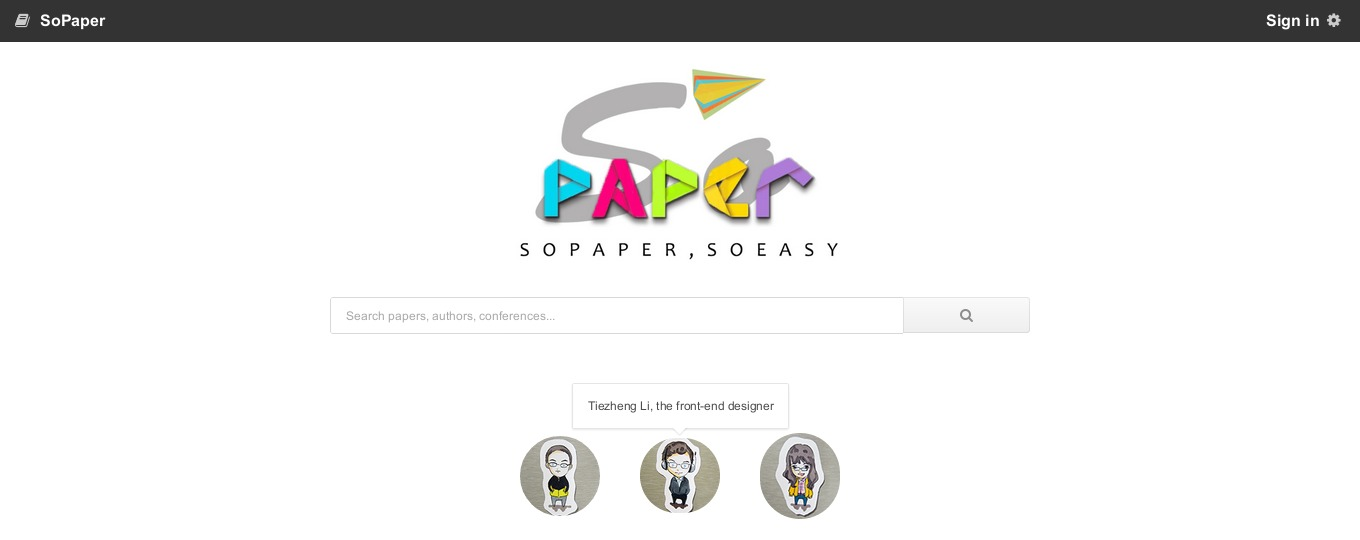
\includegraphics[width=11cm]{img/index.png}
  \caption{主页设计}
\end{figure}

主页采取搜索框居中大气简洁式设计.页面下方为作者的漫画化形象.

\begin{figure}[H]
  \small
  \centering
  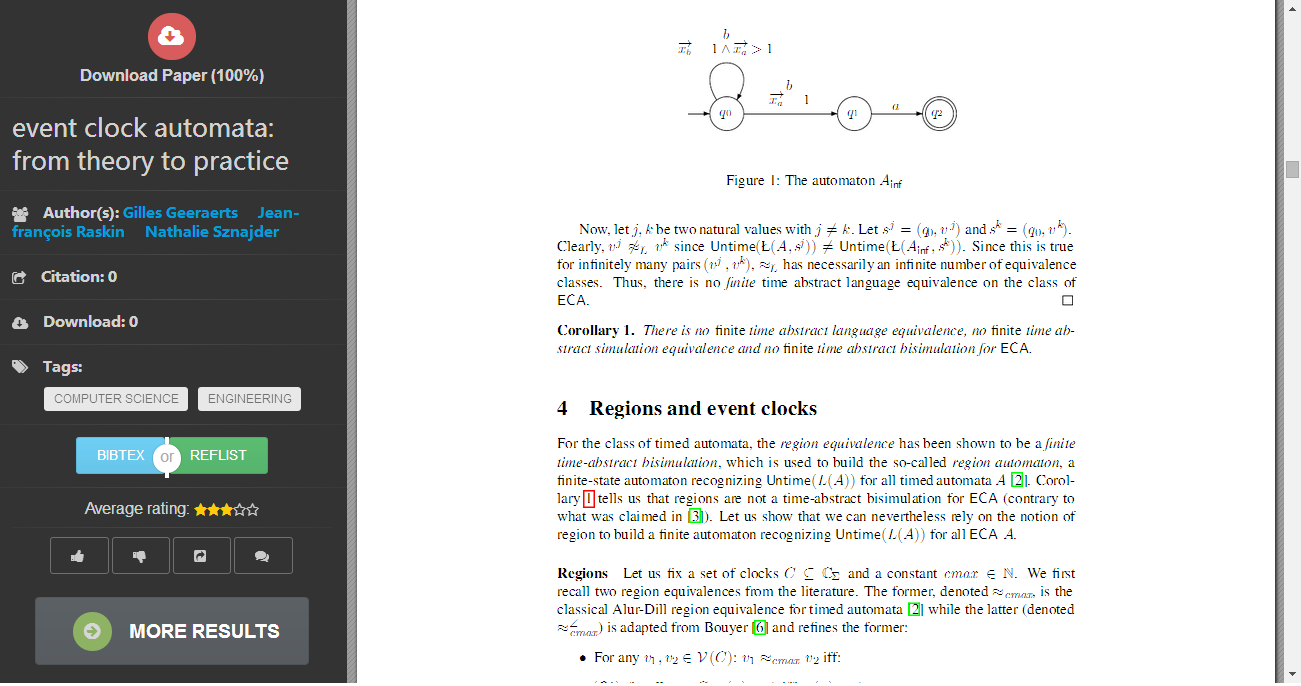
\includegraphics[width=11cm]{img/reading.png}
  \caption{阅读页面设计}
\end{figure}
可直接阅读的论文位于页面正中,左侧栏显示垂直搜索信息,包括作者、引用量、下载量、标签、引用列表等,以及提供下载、评论、分享等相关功能 按钮.

\begin{figure}[H]
  \small
  \centering
  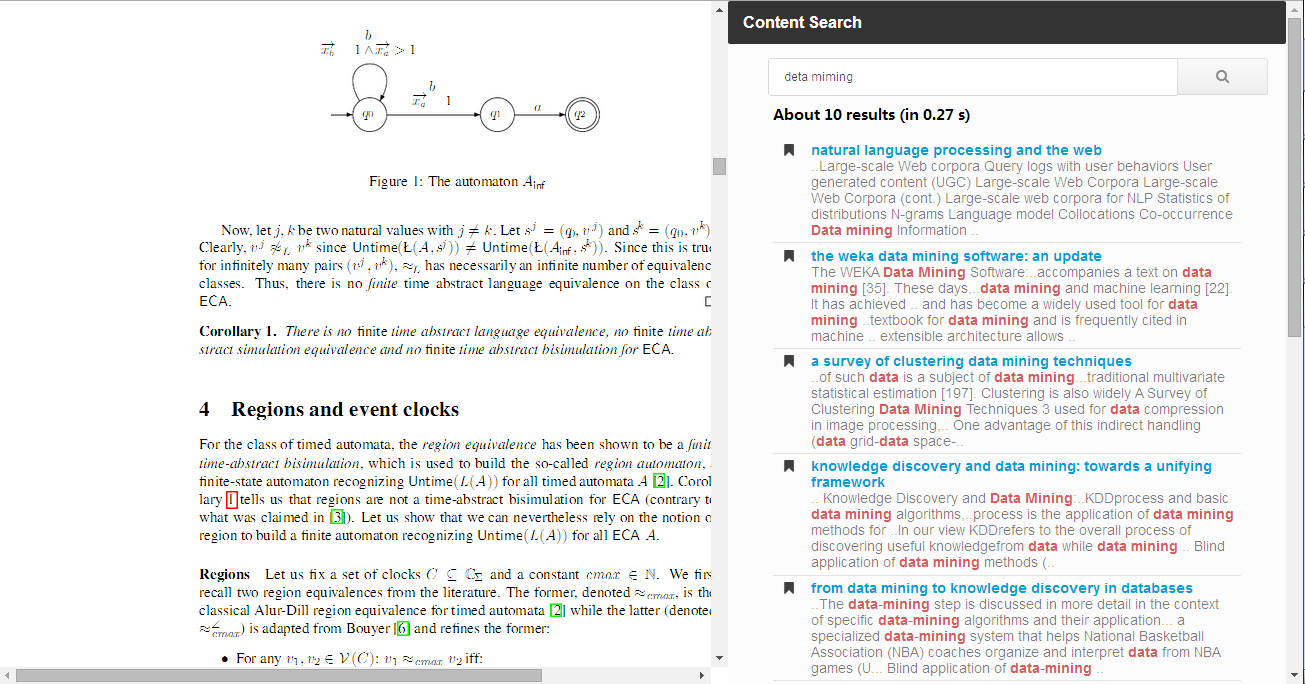
\includegraphics[width=11cm]{img/summary.png}
  \caption{摘要页面设计}
\end{figure}

摘要页面位于页面右侧栏,单个摘要包含标题及高亮关键字的正文摘要.

\begin{figure}[H]
  \small
  \centering
  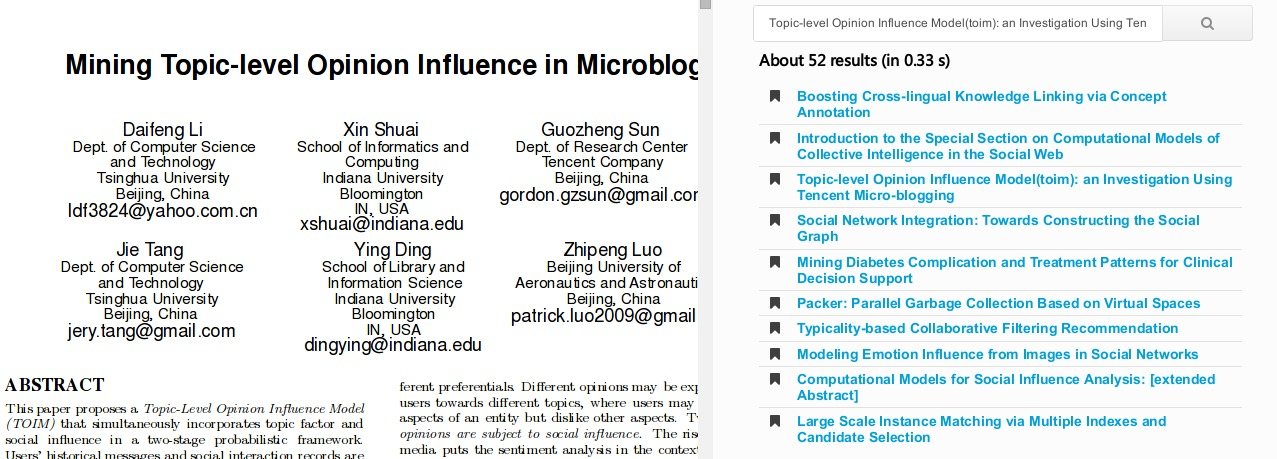
\includegraphics[width=11cm]{img/author.png}
  \caption{作者搜索}
\end{figure}


\begin{figure}[H]
  \small
  \centering
  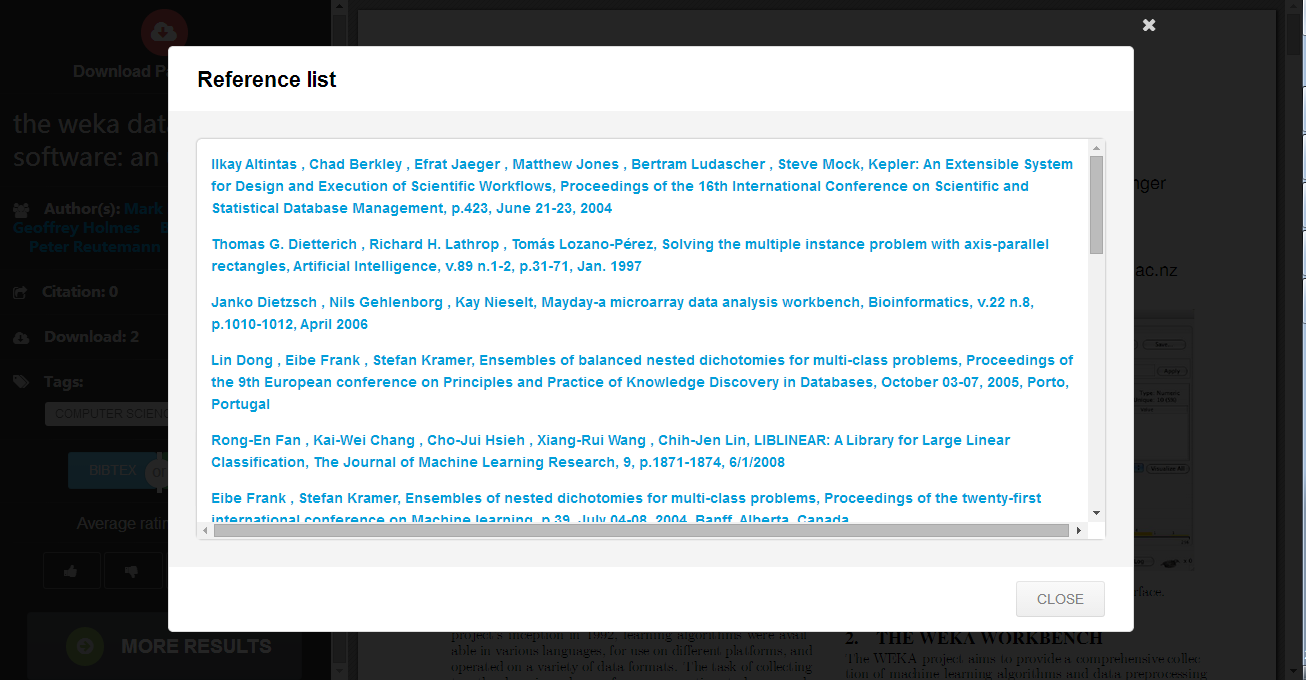
\includegraphics[width=11cm]{img/reference.png}
  \caption{论文引用情况}
\end{figure}

采用了弹出式的Modal,点击链接可直接转到引用源网页.

\subsection{交互设计}

相较于传统的搜索引擎交互模式,Sopaper做出了一些改变性的尝试:
\begin{itemize}
  \item \textbf{论文为主}:在交互上,将搜索的单个内容本身而非摘要列表作为搜索引擎的默认主体呈现内容.
  \item \textbf{立即阅读}: 提供在网页上直接阅读论文的功能.将 PDF 文件精确转换成可供 Firefox、Google Chrome 等现代浏览器直接浏览的 HTML 文件.用户无须点选,下载等复杂操作便可直接阅读论文,以便用户以最快速度是否是自己想找的论文,简要浏览论文内容,在论文中摘录信息等需求.
  \item \textbf{最大似然匹配} :当用户检索的结果可以精确的匹配到某论文的标题时,Sopaper将不返回结果的拍循序列表,而是直接进入该最有可能paper的阅读模式.跳过选择, 令用户尽可能的直达自己想要的搜索结果.
\end{itemize}


\section{总结}
由于开发团队有长期合作的经验,且分工明确,通力合作,最终成功完
成了项目.另外,这次课程设计的经历在开发之外也给我们带来了许 多宝贵的体验和教育.

整个项目的出发点简单而明确,就是要整合和改进分散、繁琐的下载流程,提供一个便捷的定
位、下载与阅读服务.消灭用户在各种页面之间手动切换、反复确认、 重命名、同步数据的
冗余工作.

如何能够删繁就简,我们两人开动脑筋设计了许多新颖的产品交互形式.经过激烈的几次讨论
,设计会,以及寻找身边同学做调研,最终决定了这样一种形式,我们在这一推敲的过程中体验到了在构建易用的产品时,苛求细节,反复迭代打磨
的工匠情怀.

目前的Sopaper还有许多待完善之处,如受到下载限制和版权限制的索引量还仍需尽可能的提
高,如收集到了论文的引用关系,用户的评论与反馈后,还可以 尝试基于此做更多的引用关系
分析,专家推荐,内容推荐等工作.有待日后的学习与研究中进一步完善.
